\chapter{Apresentação dos Resultados}

Nesta seção estão apresentados os resultados obtidos em relação à arquitetura, documentação, testes, usabilidade e
validação dos resultados entregues pela ferramenta.
Para realizar a validação dos resultados, foram feitas comparações com casos da bibliografia, com dados de experimentos
práticos já realizados e também a aplicação em um sistema real.


\section{Arquitetura}
Com o Desenvolvimento do projeto a arquitetura geral das classes se manteve.
Contudo, os métodos já existentes foram melhor definidos, além de serem adicionados diversos outros.
A estrutura geral do diagrama pode ser visualizada na figura \ref{fig:class_diag_new} e os detalhes nas figuras
\ref{fig:class_diag_diubmi_new}, \ref{fig:class_diag_du_new}, \ref{fig:class_diag_pu_new},
\ref{fig:class_diag_model_new}, \ref{fig:class_diag_controller_new} e \ref{fig:class_diag_bcacontroller_new} .

\begin{figure}[H]
    \centering
    \caption{Novo diagrama de classes}
    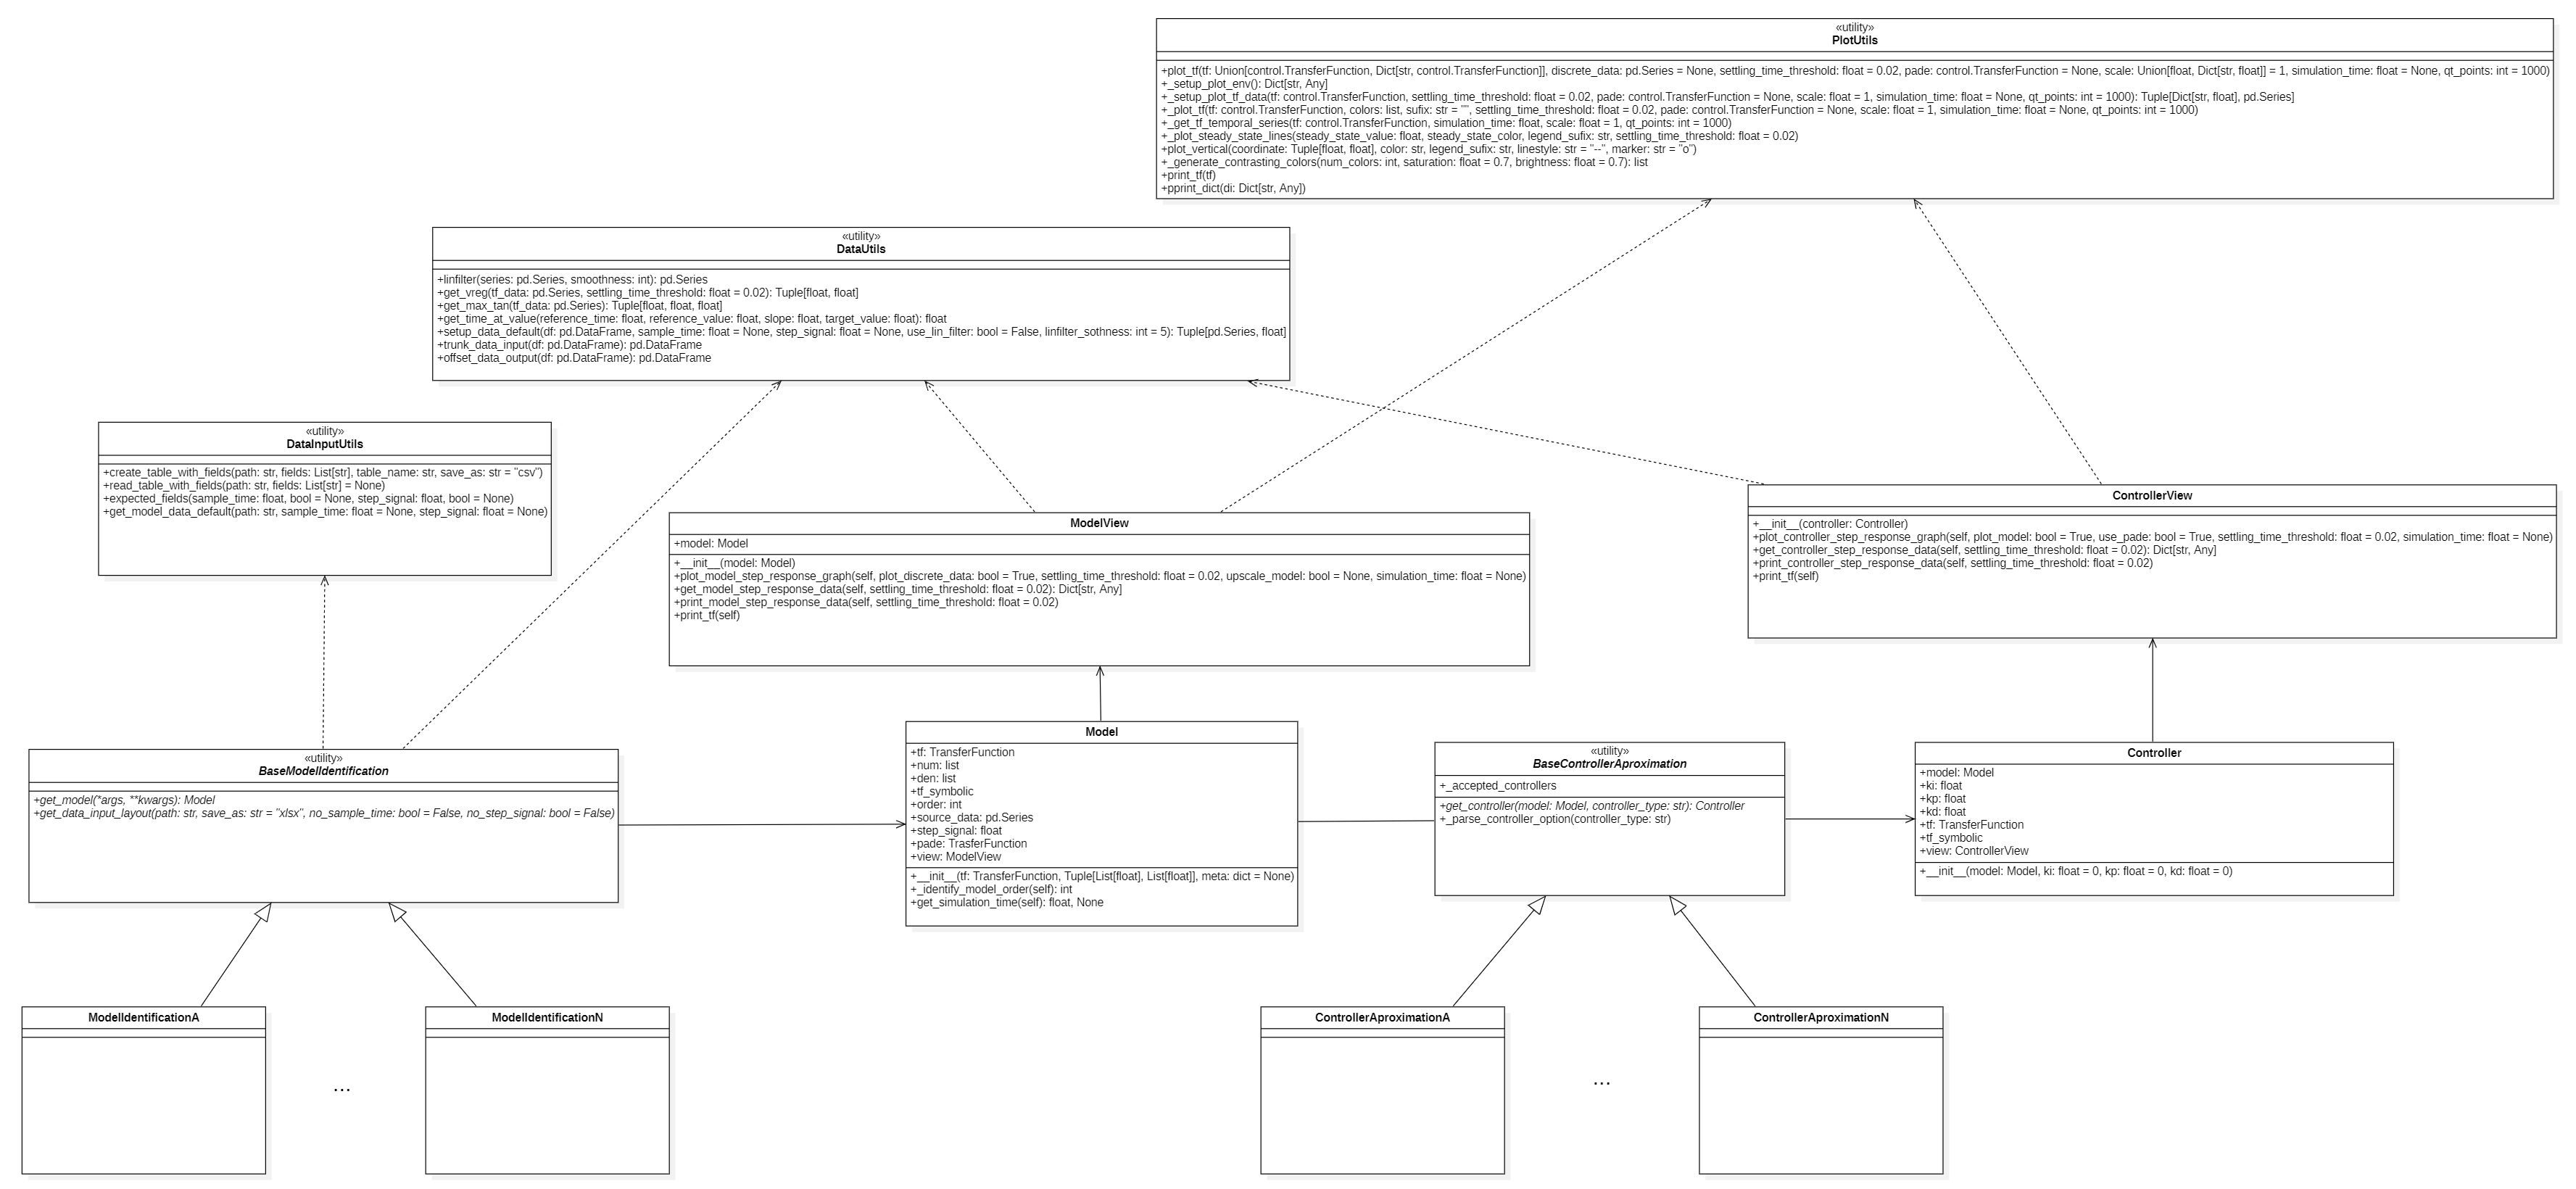
\includegraphics[scale=0.17]{figuras/class_diag_new}
    \label{fig:class_diag_new}
    \\
    \vspace{0cm}\hspace{0cm}\small{Fonte: Do autor}
\end{figure}

\begin{figure}[H]
    \centering
    \caption{Novo diagrama de classes ampliado - DataInputUtils e BaseModelIdentification}
    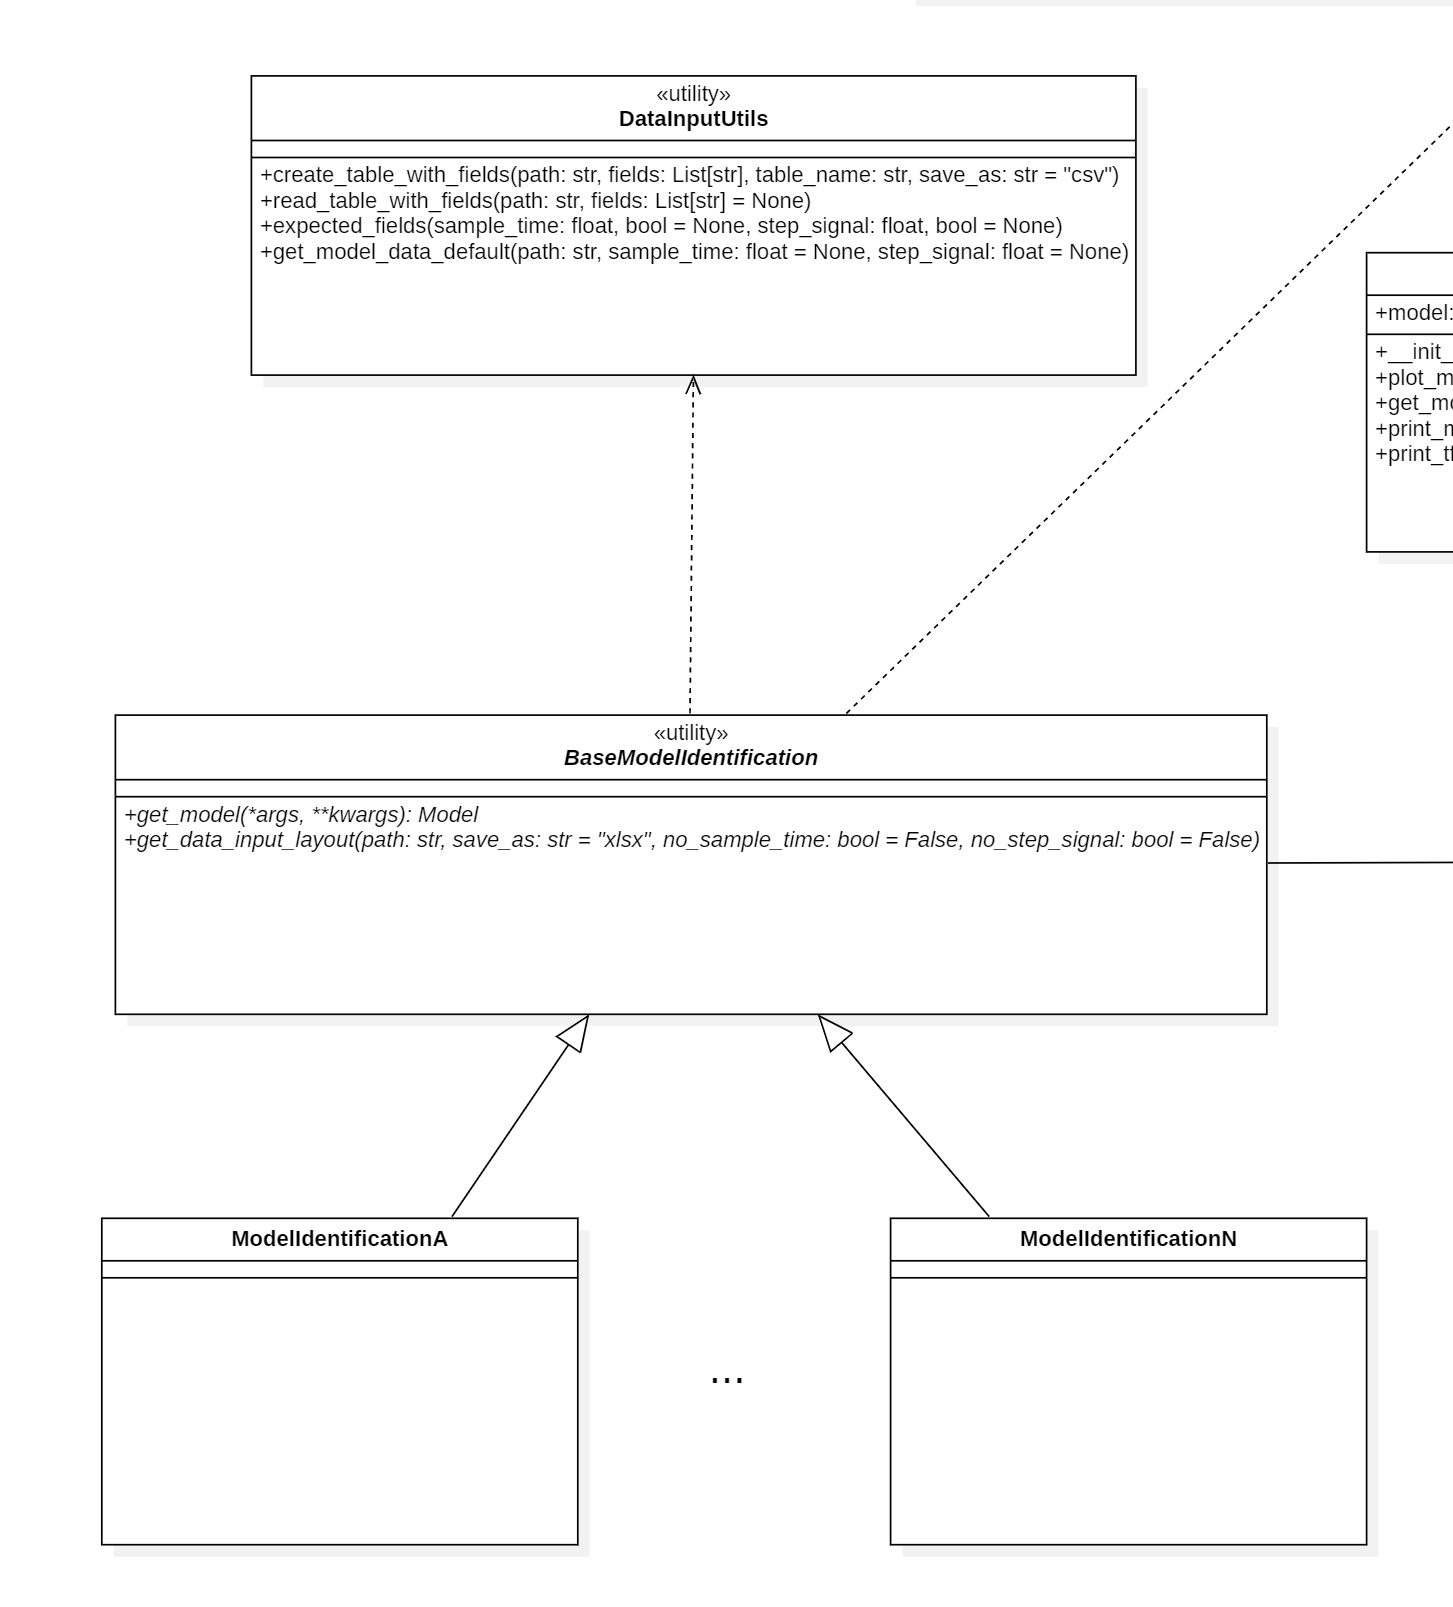
\includegraphics[scale=0.35]{figuras/class_diag_diubmi_new}
    \label{fig:class_diag_diubmi_new}
    \\
    \vspace{0cm}\hspace{0cm}\small{Fonte: Do autor}
\end{figure}

\begin{figure}[H]
    \centering
    \caption{Novo diagrama de classes ampliado - DataUtils e PlotUtils}
    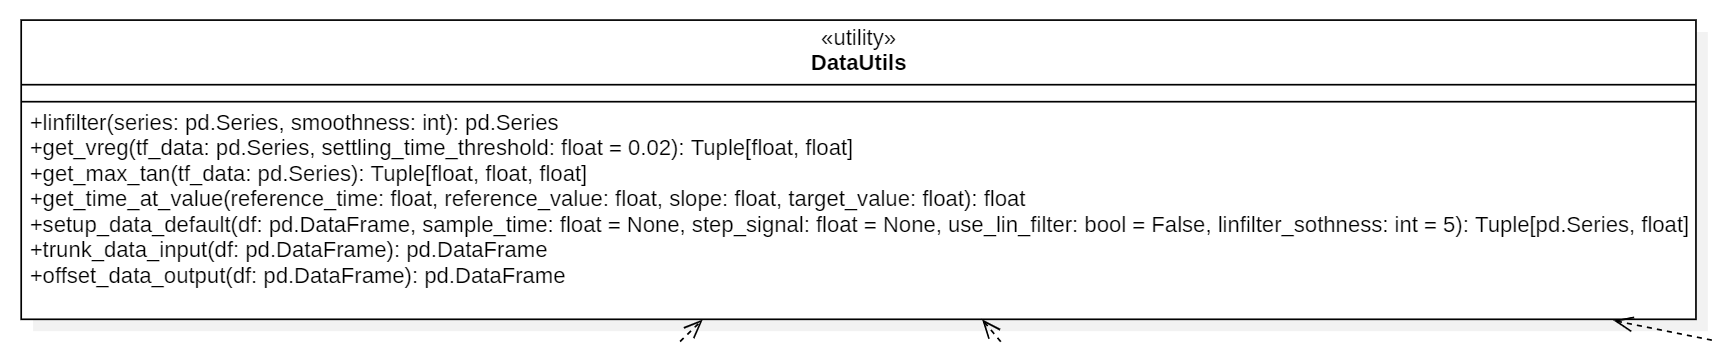
\includegraphics[scale=0.35]{figuras/class_diag_du_new}
    \label{fig:class_diag_du_new}
    \\
    \vspace{0cm}\hspace{0cm}\small{Fonte: Do autor}
\end{figure}

\begin{figure}[H]
    \centering
    \caption{Novo diagrama de classes ampliado - DataUtils e PlotUtils}
    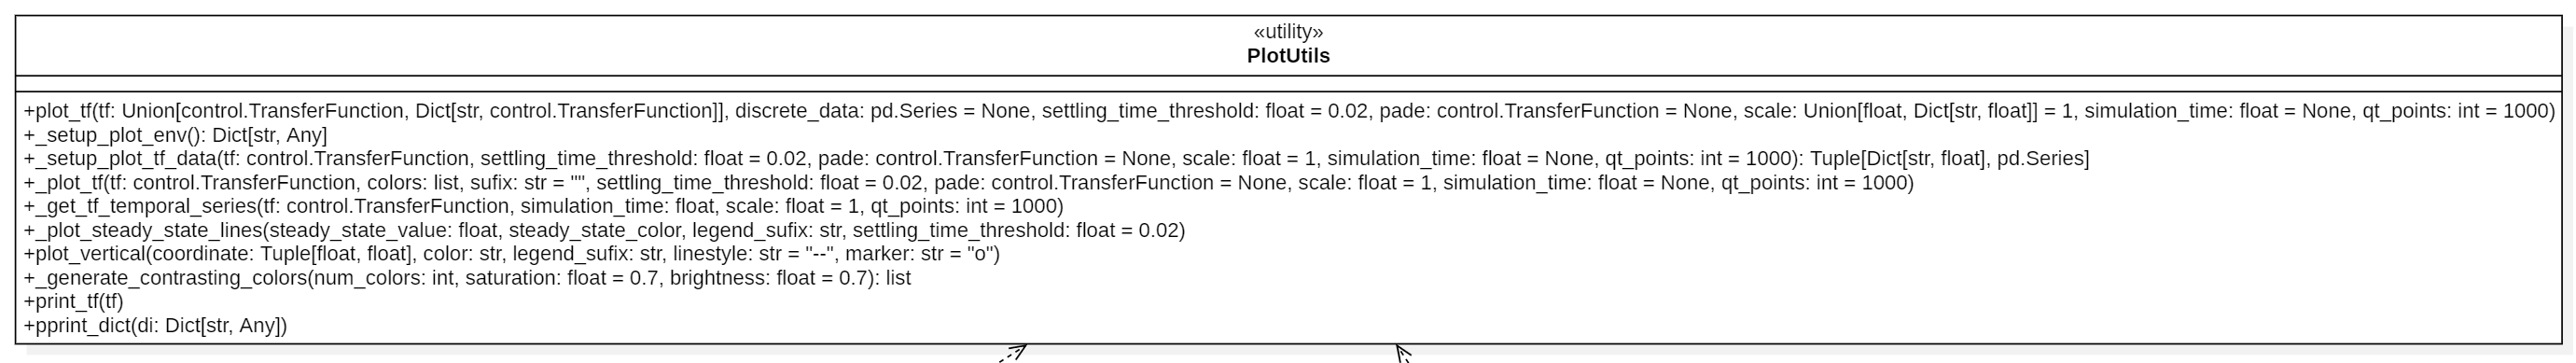
\includegraphics[scale=0.22]{figuras/class_diag_pu_new}
    \label{fig:class_diag_pu_new}
    \\
    \vspace{0cm}\hspace{0cm}\small{Fonte: Do autor}
\end{figure}

\begin{figure}[H]
    \centering
    \caption{Novo diagrama de classes ampliado - Model e ModelView}
    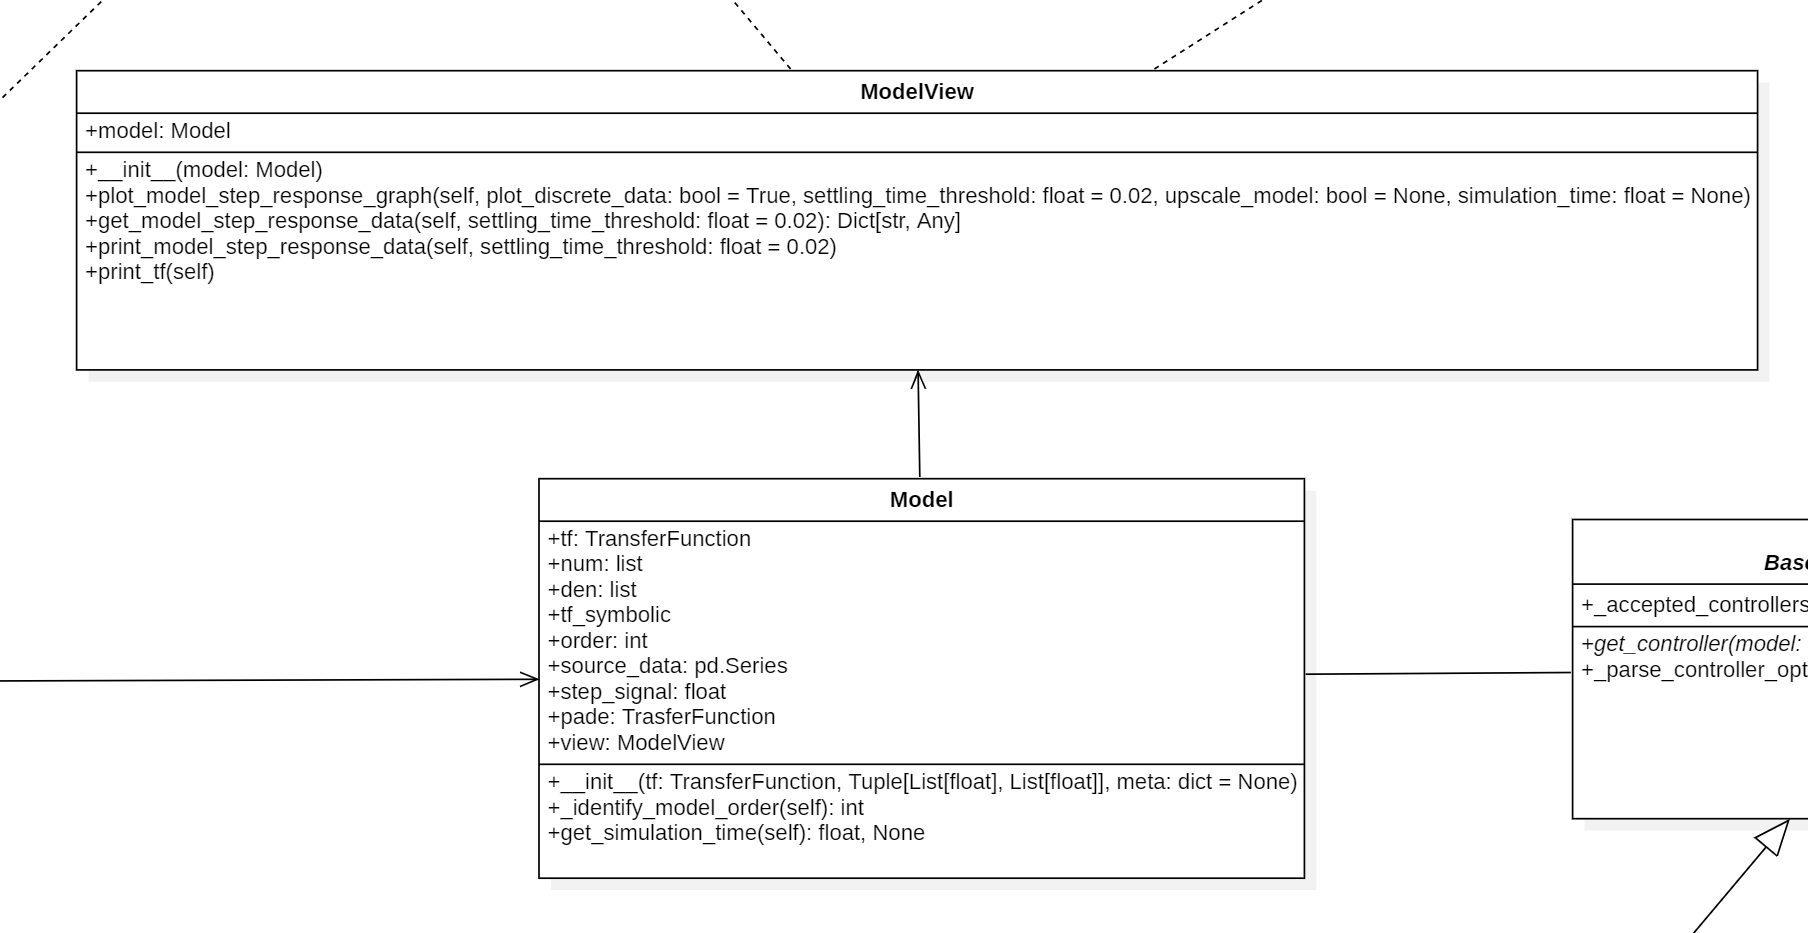
\includegraphics[scale=0.32]{figuras/class_diag_model_new}
    \label{fig:class_diag_model_new}
    \\
    \vspace{0cm}\hspace{0cm}\small{Fonte: Do autor}
\end{figure}

\begin{figure}[H]
    \centering
    \caption{Novo diagrama de classes ampliado - Controller e ControllerView}
    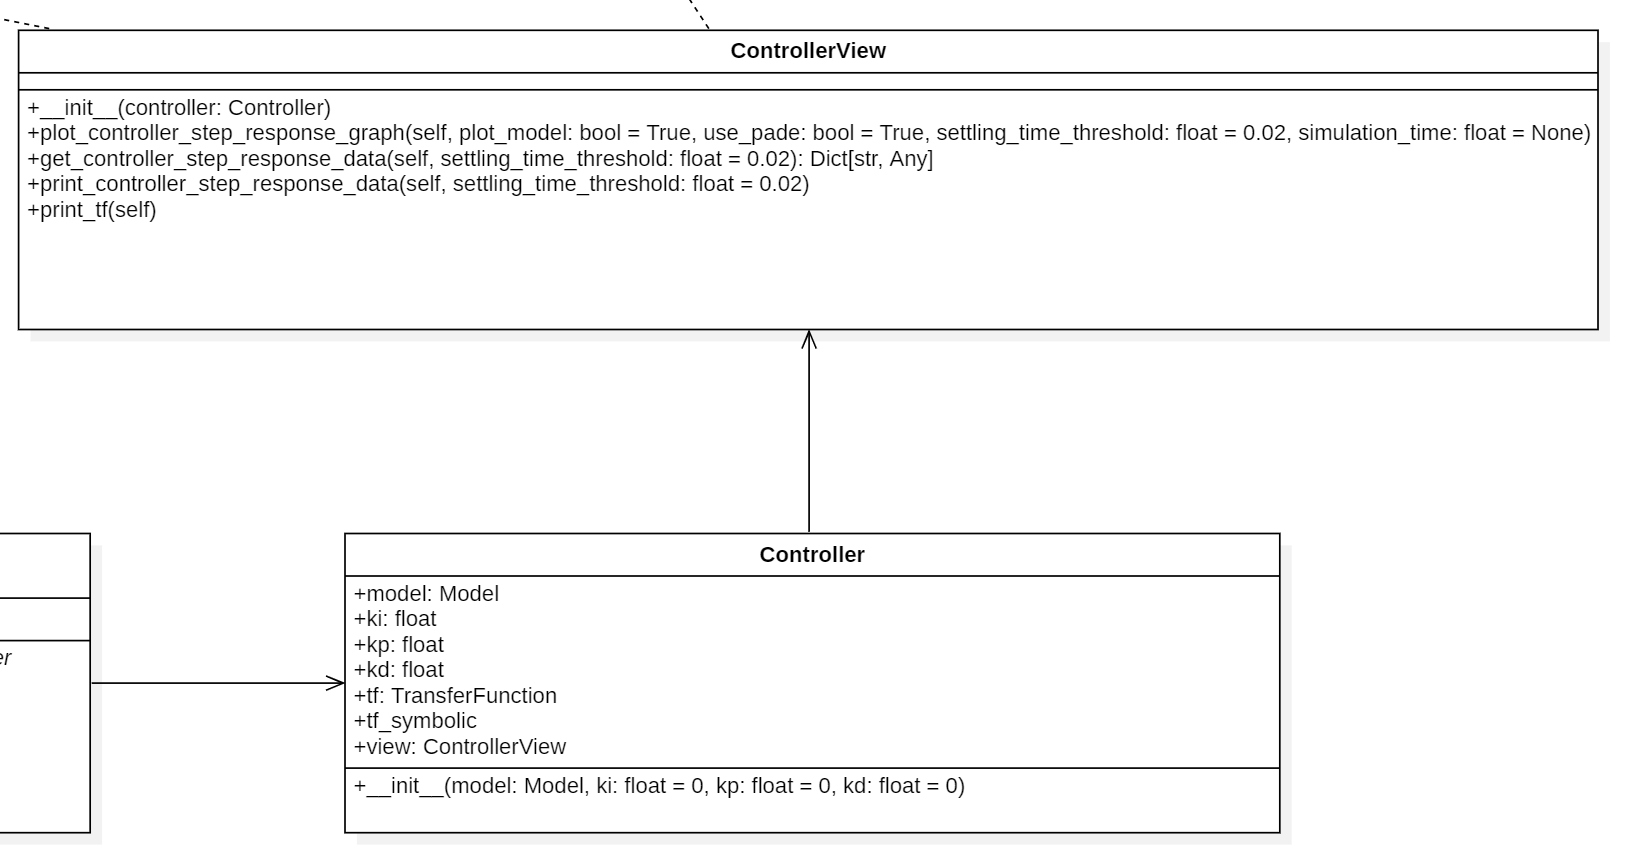
\includegraphics[scale=0.35]{figuras/class_diag_controller_new}
    \label{fig:class_diag_controller_new}
    \\
    \vspace{0cm}\hspace{0cm}\small{Fonte: Do autor}
\end{figure}

\begin{figure}[H]
    \centering
    \caption{Novo diagrama de classes ampliado - BaseControllerAproximation}
    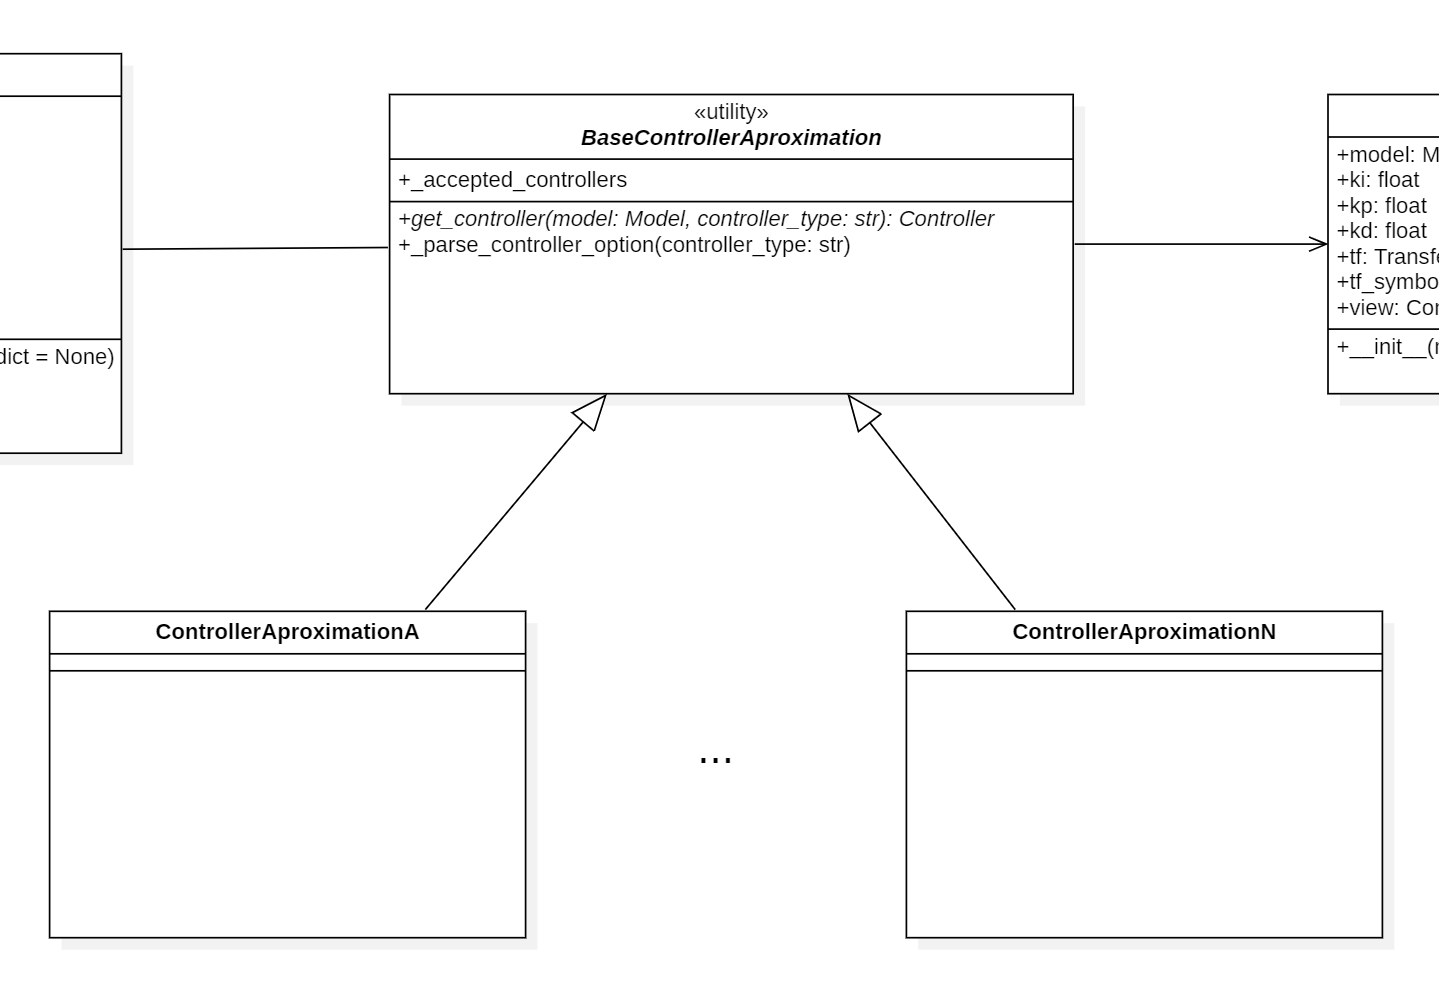
\includegraphics[scale=0.40]{figuras/class_diag_bcacontroller_new}
    \label{fig:class_diag_bcacontroller_new}
    \\
    \vspace{0cm}\hspace{0cm}\small{Fonte: Do autor}
\end{figure}


\section{Documentação}

A documentação desenvolvida juntamente a biblioteca foi compilada com sucesso e disponibilizada no link apresentado
no apêndice \ref{ch:actdocs}.
Ela abrange todas as classes implementadas bem como uma visão ampla da biblioteca e um guia rápido, além de possuir
explicações didáticas sobre o funcionamento de cada método implementado com referências bibliográficas.


\section{Testes}

Foi realizado o desenvolvimento de testes para a maioria das funcionalidades da biblioteca, ajudando na detecção
rápida de novos bugs e facilitando futuras implementações.
Uma boa parte do código desenvolvido foi coberto por esses testes, como pode ser visto na figura \ref{fig:coverage}.

\begin{figure}[H]
    \centering
    \caption{Visualização do relatório de cobertura}
    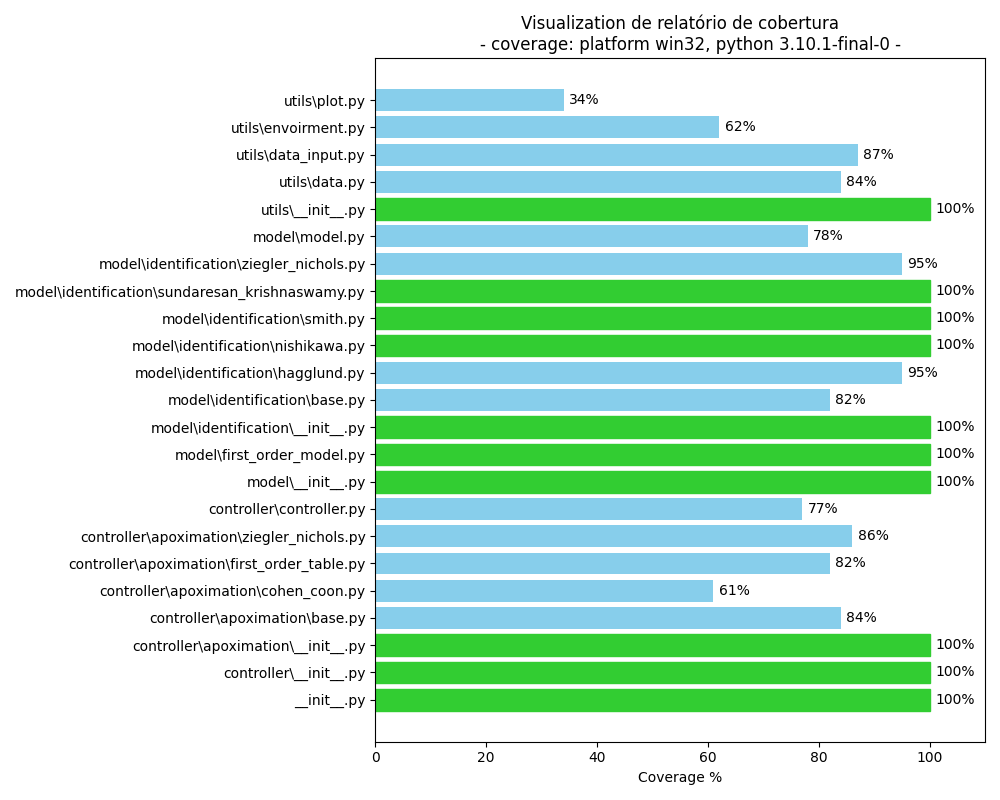
\includegraphics[scale=0.6]{figuras/coverage}
    \label{fig:coverage}
    \\
    \vspace{0cm}\hspace{0cm}\small{Fonte: Do autor}
\end{figure}


\section{Usabilidade}

A biblioteca foi projetada para um uso ágil e simples, de forma que com poucas linhas de código é possível realizar a
identificação de um modelo e a aproximação de ganhos de um controlador, bem como obter informações de suas respostas
a sinal degrau e gráficos para visualização.

Para um caso onde se deseja identificar o modelo de uma planta através do método de Nishikawa e obter um controlador
pelo método de Cohen e Coon, o primeiro paço é importar a biblioteca e obter o leiaute para entrada dos dados:

\begin{lstlisting}[label={lst:get_dil}]
import auto_control_tools as act

act.NishikawaModelIdentification.get_data_input_layout('./', save_as='csv', no_sample_time=True)
\end{lstlisting}

Com isso um arquivo \("\)data\_input.csv\("\) será criado no diretório atual.
Os dados de resposta do sistema devem ser inseridos nele, nesse caso no formato CSV, com os dados separados por vírgula.
O parâmetro no\_sample\_time foi marcado como verdadeiro, indicando para o método de criação do leiaute que não
se deseja informar os dados de tempo de aquisição na planilha fornecida.
Esse dado pode ser fornecido posteriormente como uma constante.

Com o arquivo preenchido com os dados de resposta a sinal degrau do sistema, é possível realizar a identificação,
obtendo um modelo do qual já podemos visualizar os dados e o gráfico de forma simples, como pode ser visto no trecho
de código a seguir:

\begin{lstlisting}[label={lst:get_model}]
import auto_control_tools as act

# act.NishikawaModelIdentification.get_data_input_layout('./', save_as='csv', no_sample_time=True)

model = act.NishikawaModelIdentification.get_model('./data_input.csv', sample_time=1, ignore_delay_threshold=0)

model.view.print_tf()
model.view.print_model_step_response_data()
model.view.plot_model_step_response_graph()
\end{lstlisting}

Para os dados fornecidos, a execução do código imprime as seguintes informações no terminal:
\begin{lstlisting}[label={lst:get_model_out}]
0.841304347826087*exp(-2.22428940568476*s)/(7.60658914728682*s + 1.0)
{'Overshoot': 0,
 'Peak': 0.841304292382592,
 'PeakTime': 128.0,
 'RiseTime': 16.726793943383804,
 'SettlingMax': 0.8413043478260871,
 'SettlingMin': 0.7574087299857988,
 'SettlingTime': 32.02106649111257,
 'SteadyStateValue': 0.8413043478260871,
 'Undershoot': 0.6269523372311043}
\end{lstlisting}

Além disso é aberta uma janela interativa, onde pode ser comparado o resultado da identificação com os dados de entrada
como pode ser visto na figura \ref{fig:get_model_plot}.
Nesse caso a resposta do modelo está sendo redimensionada em relação ao valor do setpoint, para ser possível a
comparação com os dados de entrada.

\begin{figure}[H]
    \centering
    \caption{Exemplo de uso da biblioteca - plot\_model\_step\_response\_graph}
    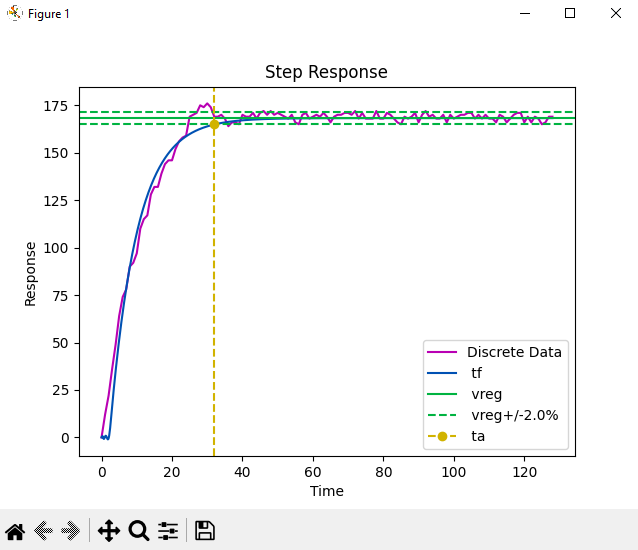
\includegraphics[scale=0.6]{figuras/get_model_plot}
    \label{fig:get_model_plot}
    \\
    \vspace{0cm}\hspace{0cm}\small{Fonte: Do autor}
\end{figure}

O processo de aproximação de ganhos de controlador por Cohen Coon ocorre de forma ainda mais simples, apenas é
necessário fornecer o modelo e o controlador desejado, a etapa de visualização de dados ocorre de forma
idêntica como pode ser visto no trecho de código a seguir:

\begin{lstlisting}[label={lst:get_controller}]
controller = act.CohenCoonControllerAproximation.get_controller(model, act.PID)

controller.view.print_tf()
controller.view.print_controller_step_response_data()
controller.view.plot_controller_step_response_graph()
\end{lstlisting}

Como pode ser visto na sequência, a execução produz uma saida idêntica no terminal, mas agora para o sistema em malha
fechada com o controlador gerado:

\begin{lstlisting}[label={lst:get_controller_out}]
0.841304347826087*(0.768000555728862*s + 5.71697021219369 + 4.89459279701174/s)*exp(-2.22428940568476*s)/((1 + 0.841304347826087*(0.768000555728862*s + 5.71697021219369 + 4.89459279701174/s)*exp(-2.22428940568476*s)/(7.60658914728682*s + 1.0))*(7.60658914728682*s + 1.0))
{'Kd': 0.7680005557288616,
 'Ki': 4.89459279701174,
 'Kp': 5.716970212193688,
 'Overshoot': 22.98302475453806,
 'Peak': 1.2298302475453806,
 'PeakTime': 5.9407504937458855,
 'RiseTime': 1.6853192890059248,
 'SettlingMax': 1.2298302475453806,
 'SettlingMin': 0.9145088850141698,
 'SettlingTime': 12.850559578670177,
 'SteadyStateValue': 1.0,
 'Undershoot': 7.829211261071754}
\end{lstlisting}

O gráfico de resposta plotado por padrão também traz a resposta do modelo em malha aberta para comparação.
Esse comportamento pode ser alterado informando o parâmetro plot\_model como False.
O resultado da plotagem pode ser visto na figura \ref{fig:get_controller_plot}.

\begin{figure}[H]
    \centering
    \caption{Exemplo de uso da biblioteca - plot\_controller\_step\_response\_graph}
    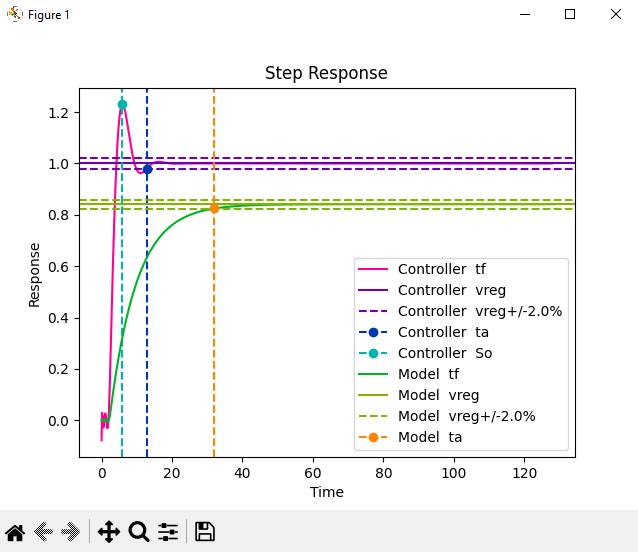
\includegraphics[scale=0.6]{figuras/get_controller_plot}
    \label{fig:get_controller_plot}
    \\
    \vspace{0cm}\hspace{0cm}\small{Fonte: Do autor}
\end{figure}

Adicionalmente, a janela interativa suporta ampliar o gráfico, para melhor visualização da resposta do sistema em
malha fechada, por exemplo.
Uma vista ampliada pode ser observada na figura \ref{fig:get_controller_plot_zoom}.

\begin{figure}[H]
    \centering
    \caption{Exemplo de uso da biblioteca - plot\_controller\_step\_response\_graph - Zoom}
    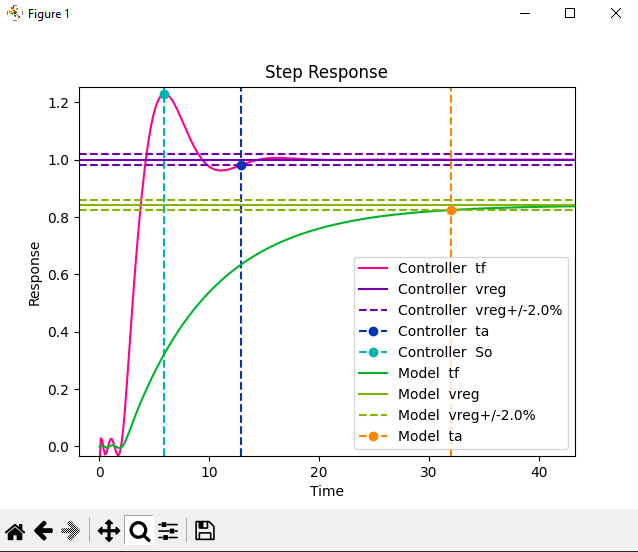
\includegraphics[scale=0.6]{figuras/get_controller_plot_zoom}
    \label{fig:get_controller_plot_zoom}
    \\
    \vspace{0cm}\hspace{0cm}\small{Fonte: Do autor}
\end{figure}

As mesmas operações podem ser executadas em qualquer ambiente com uma versão de Python suportada, inclusive em
ambientes Jupyter.
A seguir, nas figuras \ref{fig:colab_example1}, \ref{fig:colab_example2} e \ref{fig:colab_example3}, é demonstrada a
execução do mesmo código do exemplo anterior, mas desta vez no Google Colab, um serviço gratuito da empresa Google que
permite escrever e executar código Python através do navegador em um ambiente baseado em Jupyter.
Além de estar sendo executado em nuvem, o ambiente baseado em Jupyter possibilita uma formatação mais visualmente
agradável das funções de transferência e das informações de resposta a sinal degrau.

\begin{figure}[H]
    \centering
    \caption{Exemplo de uso da biblioteca - execução no colab - instalação importação e obtenção de leiaute}
    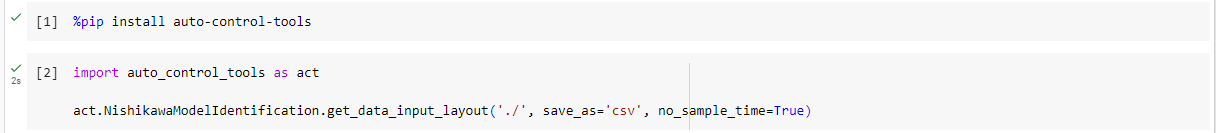
\includegraphics[scale=0.5]{figuras/colab_example1}
    \label{fig:colab_example1}
    \\
    \vspace{0cm}\hspace{0cm}\small{Fonte: Do autor}
\end{figure}

\begin{figure}[H]
    \centering
    \caption{Exemplo de uso da biblioteca - execução no colab - obtenção e visualização de modelo}
    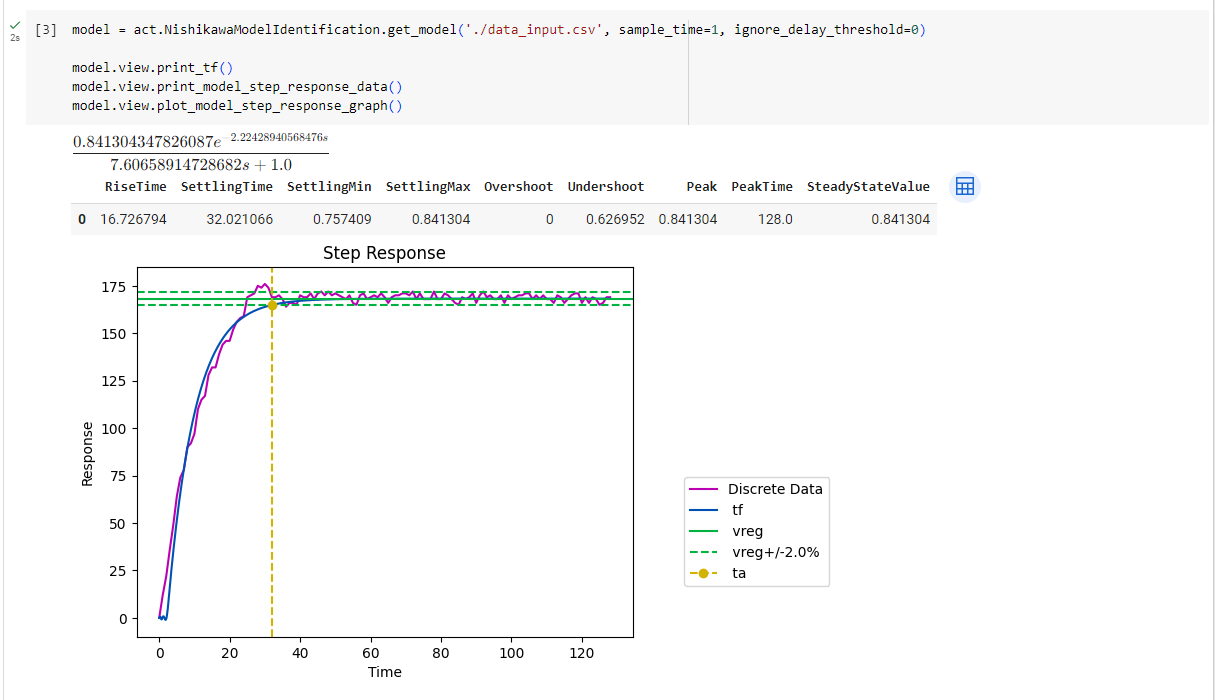
\includegraphics[scale=0.5]{figuras/colab_example2}
    \label{fig:colab_example2}
    \\
    \vspace{0cm}\hspace{0cm}\small{Fonte: Do autor}
\end{figure}

\begin{figure}[H]
    \centering
    \caption{Exemplo de uso da biblioteca - execução no colab - obtenção e visualização de controlador}
    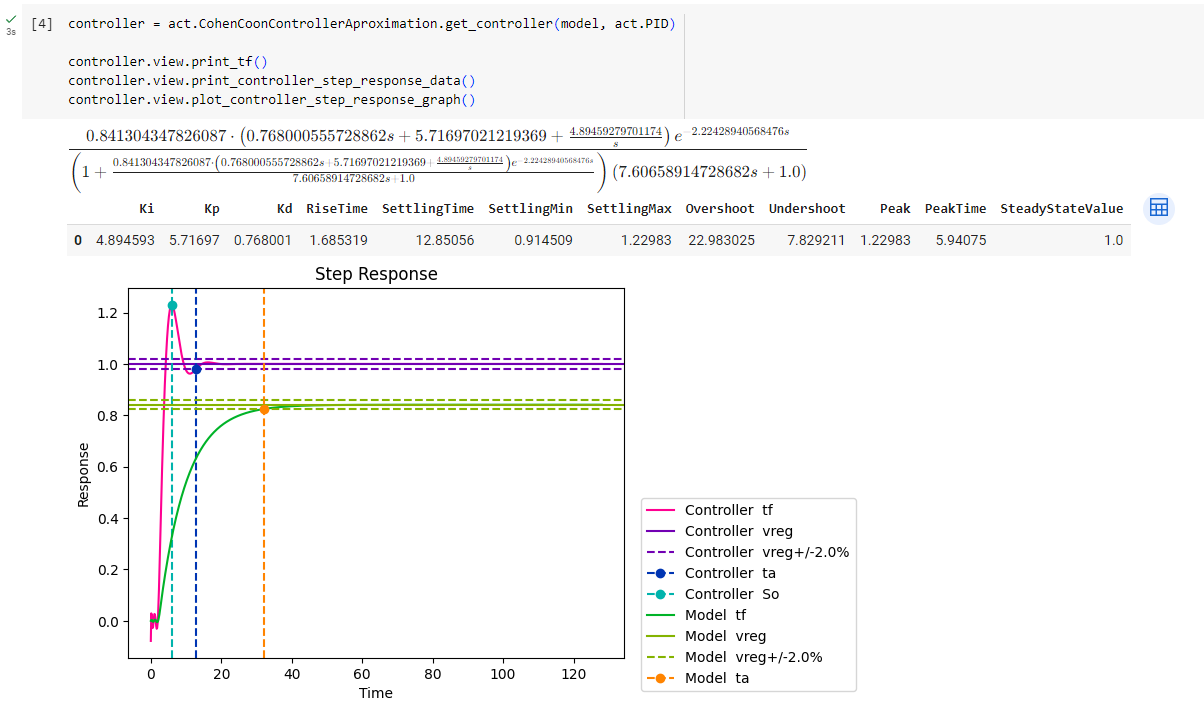
\includegraphics[scale=0.5]{figuras/colab_example3}
    \label{fig:colab_example3}
    \\
    \vspace{0cm}\hspace{0cm}\small{Fonte: Do autor}
\end{figure}


\section{Comparação com a Bibliografia}

As bibliografias de \cite{ogata2010engenharia} e \cite{CoelhoIdentificacao}, a pesar de tratarem de identificação de
modelos, não fornecem dados discretos de resposta a sinal degram para poderem ser comparados aos métodos de
identificação implementados, desta forma esta seção de comparação com a bibliografia tratará apenas dos métodos de
aproximação de ganhos de controladores PID implementados.

O primeiro caso a ser explorado será o do exemplo do tanque aquecido de \cite{apostpidsint}.
Nele é apresentado o gráfico da figura \ref{fig:bib_comp_1_graph} e determinados os parâmetros $K$, $\tau$ e $\theta$ para
obtenção do modelo clássico que a classe FirstOrderModel da seção \ref{subsubsec:fom} se especializa.
Os valores calculados podem ser vistos em \ref{eq:bib_comp_1_id} e o modelo obtido é apresentado em
\ref{eq:bib_comp_1_model}.
E os resultados da aproximação de ganhos de controlador obtidos são descritos na tabela \ref{tab:bib_comp_1_restb}.


\begin{figure}[H]
    \centering
    \caption{Curva de reação para o tanque aquecido}
    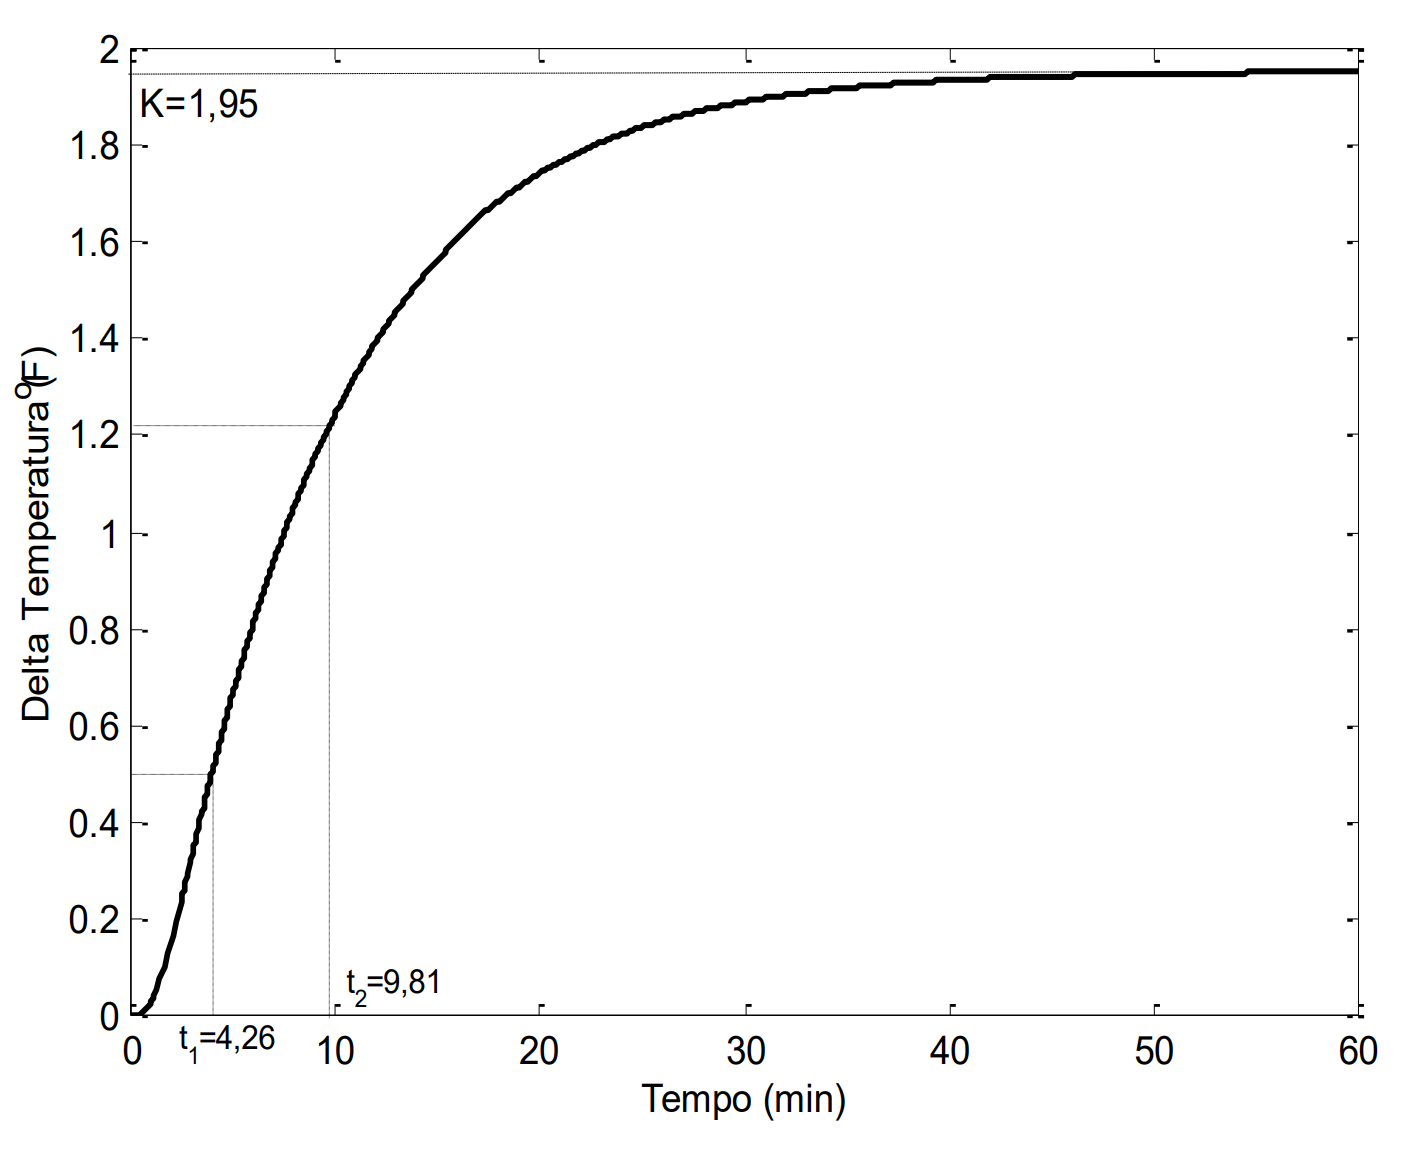
\includegraphics[scale=0.4]{figuras/bib_comp_1_graph}
    \label{fig:bib_comp_1_graph}
    \\
    \vspace{0cm}\hspace{0cm}\small{Fonte: \cite{apostpidsint}}
\end{figure}

\begin{equation}
    \label{eq:bib_comp_1_id}
    \tau = \frac{3}{2}(t_2 - t_1) = 8,33min \;\;,\;\; \theta = t_2 - T = 1,48min \;\;,\;\; K=1,95
\end{equation}

\begin{equation}
    \label{eq:bib_comp_1_model}
    G(s) = \frac{1,95}{8.33 s + 1}e^{-1,48 s}
\end{equation}

\begin{table}[h]
    \begin{center}
        \begin{tabular}{ | l | c | c | c | }
            \hline
            {}                         & {$K_P$} & {$T_I$}   & {$T_D$}   \\
            \hline
            {\textbf{Ziegler-Nichols}} & {3,46}  & {2,96min} & {0,74min} \\
            \hline
            {\textbf{Cohen-Coon}}      & {3,97}  & {3,39min} & {0,52min} \\
            \hline
        \end{tabular}
        \caption{ Métodos da curva de reação para o tanque aquecido}
        \vspace{0cm}\hspace{0cm}\small{Fonte: \cite{apostpidsint}}
        \label{tab:bib_comp_1_restb}
    \end{center}
\end{table}

Para comparação, pode-se instanciar um objeto de modelo com FirstOrderModel, utilizando os mesmos parâmetros fornecidos,
e então utilizar os métodos de aproximação de Ziegler e Nichols e de Cohen e Coon, como é disposto no trecho de código
a seguir:
\begin{lstlisting}[label={lst:bib_comp_1_code1}]
import auto_control_tools as act

model = act.FirstOrderModel(K=1.95, tau=8.33, theta=1.48)

model.view.print_tf()
model.view.print_model_step_response_data()
model.view.plot_model_step_response_graph()

controller = act.ZieglerNicholsControllerAproximation.get_controller(model, act.PID)

controller.view.print_tf()
controller.view.print_controller_step_response_data()
controller.view.plot_controller_step_response_graph()

controller = act.CohenCoonControllerAproximation.get_controller(model, act.PID)

controller.view.print_tf()
controller.view.print_controller_step_response_data()
controller.view.plot_controller_step_response_graph()
\end{lstlisting}


\section{comaprações com Experimentos Anteriores}

Compare results to previous experiments


\section{Aplicação em Sistema Real}

Use on a real system
